%\begin{frame}[t]{Test Coverage Monitoring}

  \hspace*{-.5in}
  \begin{minipage}{5in}
  \begin{center}

      \begin{minipage}{4.5in}

    \tikzstyle{proc} = [draw, thick, fill=blue!40, text centered, rounded corners]
    \tikzstyle{procpass} = [draw, thick, fill=forestgreen!50, text centered, rounded corners]
    \tikzstyle{procrun} = [draw, thick, fill=orange!40, text centered, rounded corners]
    \tikzstyle{prochighlight} = [draw, thick, fill=yellow!40, text centered, rounded corners]
    \tikzstyle{procfail} = [draw, thick, fill=red!40, text centered, rounded corners]
    \tikzstyle{procold} = [draw, thick, fill=black!40, text centered, rounded corners]

    \tikzstyle{io} = [ellipse, draw, thick, fill=blue!20]
    \tikzstyle{iopass} = [ellipse, draw, thick, fill=orange!20]
    \tikzstyle{iofail} = [ellipse, draw, thick, fill=red!30]
    \tikzstyle{iofailother} = [ellipse, draw, thick, fill=yellow!30]
    \tikzstyle{iohighlight} = [ellipse, draw, thick, fill=yellow!20]
    \tikzstyle{feature} = [draw, thick, fill=purple!40, text centered]  
    \tikzstyle{featureold} = [draw, thick, fill=black!40, text centered]
    \tikzstyle{special} = [draw, thick, fill=orange!40, text centered, rounded corners]    
    \tikzstyle{fail} = [draw, thick, fill=red!50, text centered]    

    \begin{figure}

    \begin{center}

      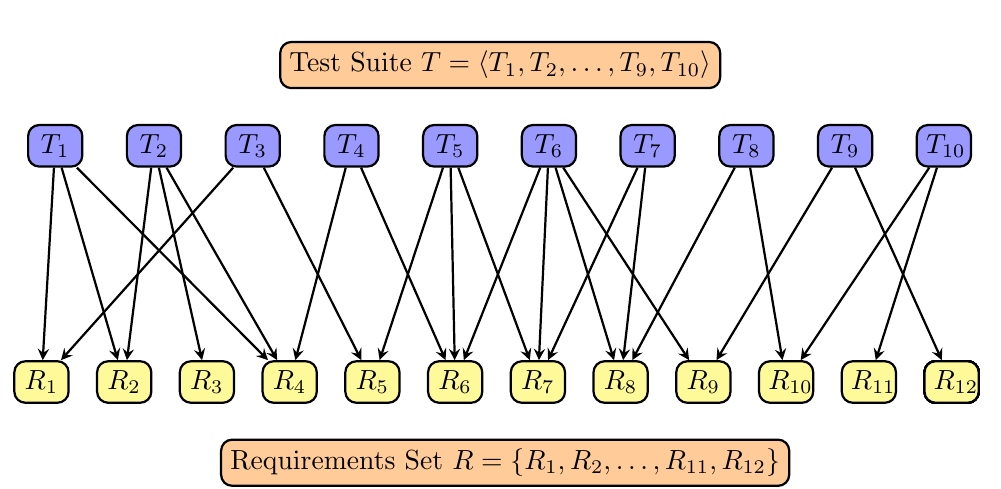
\begin{tikzpicture}[node distance=1cm, auto,>=stealth, thick]
	
        \path[use as bounding box] (-2,3.5) rectangle (10,-2);

        %%%%% 1

        % A Test Case
    	\path[->]<1-> node[proc, text width=3ex] 
        (One) at (-1.65,2.00) {$T_1$};

        % A Test Case
        \path[->]<1-> node[proc, right of=One,  
                      yshift=0in, xshift=.1in, text width=3ex] 
                      (Two) {$T_2$};

        % A Test Case
        \path[->]<1-> node[proc, right of=Two,  
                      yshift=0in, xshift=.1in, text width=3ex] 
                      (Three) {$T_3$};

        % A Test Case
        \path[->]<1-> node[proc, right of=Three,  
                      yshift=0in, xshift=.1in, text width=3ex] 
                      (Four) {$T_4$};

        % A Test Case
        \path[->]<1-> node[proc, right of=Four,  
                      yshift=0in, xshift=.1in, text width=3ex] 
                      (Five) {$T_5$};

        % A Test Case
        \path[->]<1-> node[proc, right of=Five,  
                      yshift=0in, xshift=.1in, text width=3ex] 
                      (Six) {$T_6$};

        % A Test Case
        \path[->]<1-> node[proc, right of=Six,  
                      yshift=0in, xshift=.1in, text width=3ex] 
                      (Seven) {$T_7$};

        % A Test Case
        \path[->]<1-> node[proc, right of=Seven,  
                      yshift=0in, xshift=.1in, text width=3ex] 
                      (Eight) {$T_8$};

        % A Test Case
        \path[->]<1-> node[proc, right of=Eight,  
                      yshift=0in, xshift=.1in, text width=3ex] 
                      (Nine) {$T_9$};

        % A Test Case
        \path[->]<1-> node[proc, right of=Nine,  
                      yshift=0in, xshift=.1in, text width=3ex] 
                      (Ten) {$T_{10}$};

        % Show the test suite
        \path[->]<1-> node[special, above of=Five,  
                      yshift=.01in, xshift=.25in] 
                      (TestSuite) 
              {Test Suite $T = \langle T_1, T_2, \ldots, T_9, T_{10} \rangle$};
        
        % Show the JUnit test automation framework      
        %% \path[->]<1-> node[special, below of=TestSuite,  
        %%               yshift=-.715in, xshift=0in] 
        %%               (JUnit) 
        %%       {\begin{minipage}{3.5in} \centering
        %%           JUnit and DBUnit Test Automation Frameworks \\
        %%           Database-Aware Test Coverage Monitor \\
        %%           Proteja Test Suite Manager 
        %%       \end{minipage}};

        % start running the test suite

        % A Test Case
    	%% \path[->]<1-> node[procrun, text width=3ex] 
        %% (One) at (-1.65,2.00) {$T_1$};      

        %% \path[->]<1-4> node[procrun, below of=JUnit,  
        %%               yshift=-.175in, xshift=0in] 
        %%               (Run) 
        %%       {Run Test Case};

        %% \path[->]<4-4> node[procrun, below of=Run,  
        %%               yshift=0in, xshift=0in] 
        %%               (Run) 
        %%       {Collect Per-Test Case Coverage};

        %%%%%%%%%%
              
        % Try to show the coverage report

        \path[->]<1-> node[prochighlight, text width=3ex] 
        (OneR) at (-1.825,-1.00) {$R_1$};

        \path[->]<1-> node[prochighlight, right of=OneR,  
                      yshift=0in, xshift=.02in, text width=3ex] 
                      (TwoR) {$R_2$};

        \path[->]<1-> node[prochighlight, right of=TwoR,  
                      yshift=0in, xshift=.02in, text width=3ex] 
                      (ThreeR) {$R_3$};

        \path[->]<1-> node[prochighlight, right of=ThreeR,  
                      yshift=0in, xshift=.02in, text width=3ex] 
                      (FourR) {$R_4$};

        \path[->]<1-> node[prochighlight, right of=FourR,  
                      yshift=0in, xshift=.02in, text width=3ex] 
                      (FiveR) {$R_5$};

        \path[->]<1-> node[prochighlight, right of=FiveR,  
                      yshift=0in, xshift=.02in, text width=3ex] 
                      (SixR) {$R_6$};

        \path[->]<1-> node[prochighlight, right of=SixR,  
                      yshift=0in, xshift=.02in, text width=3ex] 
                      (SevenR) {$R_7$};

        \path[->]<1-> node[prochighlight, right of=SevenR,  
                      yshift=0in, xshift=.02in, text width=3ex] 
                      (EightR) {$R_8$};

        \path[->]<1-> node[prochighlight, right of=EightR,  
                      yshift=0in, xshift=.02in, text width=3ex] 
                      (NineR) {$R_9$};

        \path[->]<1-> node[prochighlight, right of=NineR,  
                      yshift=0in, xshift=.02in, text width=3ex] 
                      (TenR) {$R_{10}$};

        \path[->]<1-> node[prochighlight, right of=TenR,  
                      yshift=0in, xshift=.02in, text width=3ex] 
                      (ElevenR) {$R_{11}$};

        \path[->]<1-> node[prochighlight, right of=ElevenR,  
                      yshift=0in, xshift=.02in, text width=3ex] 
                      (TwelveR) {$R_{12}$};

        % Show the set of requirements
        \path[->]<1-> node[special, below of=SixR,  
                      yshift=-.01in, xshift=.25in] 
                      (Requirements) 
              {Requirements Set $R = \{ R_1, R_2, \ldots, R_{11}, R_{12} \}$};

        % Granularity
        \path[->]<1-> node[special, below of=Requirements,  
                      yshift=-.01in, xshift=0in] 
                      (Granularity) 
             {Granularity varies from database to attribute value};

        % Details
        \path[->]<1-> node[special, below of=Granularity,  
                      yshift=-.01in, xshift=0in] 
                      (Reference) 
              {See [Kapfhammer and Soffa, ISEC 2008] for more details};

        % Reduction
        \path[->]<1-> node[special, below of=Reference,  
                      yshift=-.01in, xshift=0in] 
                      (Reduction) 
              {Overlap-aware test suite reduction greedily removes redundant tests};


        
        %%%%% 4

        \path[->]<1-> node[prochighlight, right of=ElevenR,  
                      yshift=0in, xshift=.02in, text width=3ex] 
                      (TwelveR) {$R_{12}$}
        (One) edge node {} (OneR)
        (One) edge node {} (TwoR)
        (One) edge node {} (FourR);

        \path[->]<1-> node[prochighlight, right of=ElevenR,  
                      yshift=0in, xshift=.02in, text width=3ex] 
                      (TwelveR) {$R_{12}$}
        (Two) edge node {} (TwoR)
        (Two) edge node {} (ThreeR)
        (Two) edge node {} (FourR);

        \path[->]<1-> node[prochighlight, right of=ElevenR,  
                      yshift=0in, xshift=.02in, text width=3ex] 
                      (TwelveR) {$R_{12}$}
        (Three) edge node {} (OneR)
        (Three) edge node {} (FiveR);

        \path[->]<1-> node[prochighlight, right of=ElevenR,  
                      yshift=0in, xshift=.02in, text width=3ex] 
                      (TwelveR) {$R_{12}$}
        (Four) edge node {} (FourR)
        (Four) edge node {} (SixR);

        \path[->]<1-> node[prochighlight, right of=ElevenR,  
                      yshift=0in, xshift=.02in, text width=3ex] 
                      (TwelveR) {$R_{12}$}
        (Five) edge node {} (FiveR)
        (Five) edge node {} (SixR)
        (Five) edge node {} (SevenR);

        \path[->]<1-> node[prochighlight, right of=ElevenR,  
                      yshift=0in, xshift=.02in, text width=3ex] 
                      (TwelveR) {$R_{12}$}
        (Six) edge node {} (SixR)
        (Six) edge node {} (SevenR)
        (Six) edge node {} (EightR)
        (Six) edge node {} (NineR);

        \path[->]<1-> node[prochighlight, right of=ElevenR,  
                      yshift=0in, xshift=.02in, text width=3ex] 
                      (TwelveR) {$R_{12}$}
        (Seven) edge node {} (SevenR)
        (Seven) edge node {} (EightR);

        \path[->]<1-> node[prochighlight, right of=ElevenR,  
                      yshift=0in, xshift=.02in, text width=3ex] 
                      (TwelveR) {$R_{12}$}
        (Eight) edge node {} (EightR)
        (Eight) edge node {} (TenR);

        \path[->]<1-> node[prochighlight, right of=ElevenR,  
                      yshift=0in, xshift=.02in, text width=3ex] 
                      (TwelveR) {$R_{12}$}
        (Nine) edge node {} (NineR)
        (Nine) edge node {} (TwelveR);

        \path[->]<1-> node[prochighlight, right of=ElevenR,  
                      yshift=0in, xshift=.02in, text width=3ex] 
                      (TwelveR) {$R_{12}$}
        (Ten) edge node {} (TenR)
        (Ten) edge node {} (ElevenR);

        % Show the set of requirements
        %% \path[->]<8-8> node[special, below of=SixR,  
        %%               yshift=-.1in, xshift=.25in] 
        %%               (Requirements) 
        %%       {Requirements Set $R$ for ... Statement Coverage};

        %% % Show the set of requirements
        %% \path[->]<9-9> node[special, below of=SixR,  
        %%               yshift=-.1in, xshift=.25in] 
        %%               (Requirements) 
        %%       {Requirements Set $R$ for ... Database Interaction Coverage};

        %% % Show the set of requirements
        %% \path[->]<10-10> node[special, below of=SixR,  
        %%               yshift=-.1in, xshift=.25in] 
        %%               (Requirements) 
        %%       {Requirements Set $R$ for ... Database Table Coverage};

        %% % Show the set of requirements
        %% \path[->]<11-11> node[special, below of=SixR,  
        %%               yshift=-.1in, xshift=.25in] 
        %%               (Requirements) 
        %%       {Requirements Set $R$ for ... Database Record Coverage};

        %% % Show the set of requirements
        %% \path[->]<12-12> node[special, below of=SixR,  
        %%               yshift=-.1in, xshift=.25in] 
        %%               (Requirements) 
        %%       {Requirements Set $R$ for ... Database Attribute Coverage};

        %% % Show the set of requirements
        %% \path[->]<13-13> node[special, below of=SixR,  
        %%               yshift=-.1in, xshift=.25in] 
        %%               (Requirements) 
        %%       {Requirements Set $R$ for ... Database Attribute-Value Coverage};

 	\end{tikzpicture}
	
        \end{center}

        \end{figure}
      
      \end{minipage} 

  \end{center}
  \end{minipage}

%\end{frame}
